%%%%%%%%%%%%%%%%%%%%%%%%%%%%%%%%%%%%
\newcommand{\setSinkAgents}[2]{\setSymbol{SG}{#1}{#2}}
\newcommand{\formalAgentResources}[2]{
	\functionFormal{ar}
	{\setAgents{}{} \times \setResource{}{}}
	{\setRealNumbersNonNegative{}{}}
}
\newcommand{\functionAgentResources}[2]{
	\functionSignature{ar}{\varAgent{}{}, \varResource{}{}}
}
\newcommand{\formalSinkMapping}[2]{
	\functionFormal{sg}
	{\setCompositeTask{}{}}
	{\powerSetSymbol{\setSinkAgents{#1}{#2}}{}{}}
}



\begin{figure}
\centering 
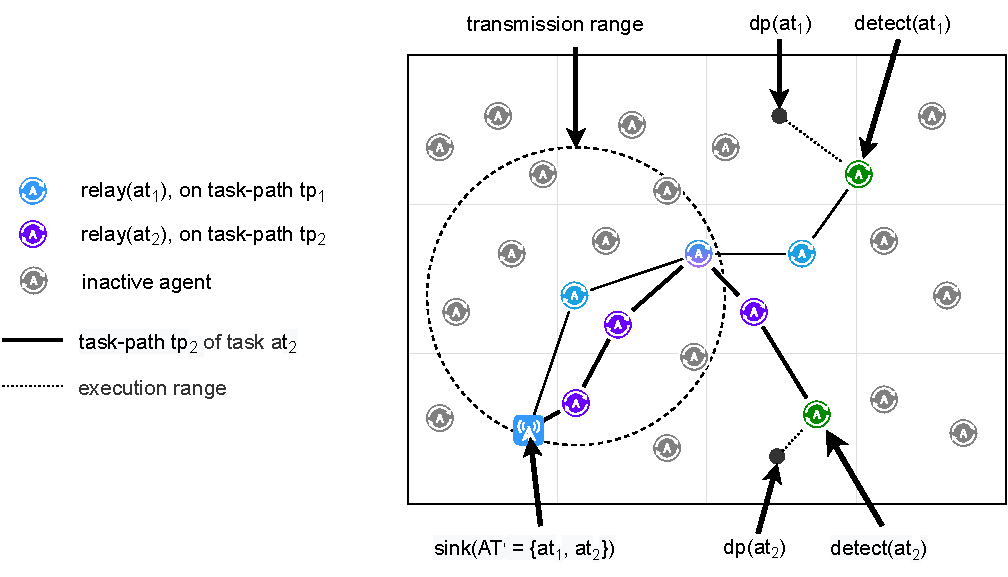
\includegraphics[width=0.9\linewidth, trim={25pt 0pt 24pt 0pt, clip}]{grid_concept}
\caption[WSN deployment terminology]{WSN components and terminology}
\label{fig:grid_concept}
\end{figure}

\subsection{Tasks and resources}

In our assumed system there is a geographical area to monitor  on which a set of agents $\setAgents{}{}$ are distributed randomly, such as occurs in an aerial deployment \citep{Kumar2013}.  The area is defined by a two dimensional grid of non-negative real numbers onto which the \textit{deployment configuration} maps each agent to a distinct location.  Agents can perform tasks, which are typed. These can be either \textit{atomic tasks}, for individual measurements, or \textit{composite tasks}, composed of a set of atomic tasks. Each atomic task targets a measurement at a location on this grid, the tasks' \textit{demand point}. Composite tasks are allocated to sink nodes throughout the systems' lifetime from an external source. These composite tasks are then decomposed into atomic tasks by the sink nodes, with each atomic task them being either executed by the node, or allocated to other nodes to complete or relay further. Completing atomic tasks requires \textit{resources}, such as energy, of which a node has a fixed amount . At any given time each node has a certain amount of its' available resources assigned to completing each type of atomic task.  We so define the system as an agent-based system formed from the tuple, $\langle 
	\setAgents{}{},
	\setSinkAgents{}{},
	\setAtomicTask{}{},
	\setCompositeTask{}{},
	\setResource{}{},
	\mathit{ar},
	\mathit{ra},
	\mathit{sg},
	\mathit{conf},
	\mathit{dp}
\rangle$, where
\begin{itemize}
	\item $\setAgents{}{}$ is a set of agents in the system that can complete tasks;
	\item $\setSinkAgents{}{} \subset \setAgents{}{}$ is a set of sink nodes, agents that can receive composite tasks from external to the system;
	\item $\setAtomicTask{}{}$ is a set of atomic tasks where each task is a measurement task performed by a single agent;
	\item $\setCompositeTask{}{} \subseteq \powerSetSymbol{\setAtomicTask{}{}}{}{}$ is the set of composite tasks that occur in the system;
	\item $\setResource{}{}$ is a set of resources needed to perform atomic tasks;
	  \item $\formalAgentResources{}{}$ is a mapping from each agent and each resource to the amount of that resource that the agent possesses.
	 \item $\formalTaskResourceAllocation{}{}$ maps each agent and type of atomic task, to a value representing the amount of a resource it has assigned to completing tasks of that type.
	\item $\formalSinkMapping{}{}$ is a static mapping from each composite task type to the group of sink agents that receive and ensure the completion of tasks of that type, fixed on system initialisation.
	\item $\formalDeployment{}{}$ is a mapping of each agent to their location in the system.
	\item  $\formalTaskDemandPoint{}{}$ maps atomic tasks to their respective demand points.
\end{itemize}

\subsection{Node roles and task paths}
%%%%%%%%%%%%%%%%%%%%%%%%%%%%%%%%%%%%%%%%%%%%
\newcommand{\formalSinkRole}[2]{
	\functionFormal{sink}
	{\setAtomicTask{}{}}
	{\setAgents{}{}}
}
\newcommand{\formalSenseRole}[2]{
	\functionFormal{sensor}
	{\setAtomicTask{}{}}
	{\setAgents{}{}}
}
\newcommand{\formalActiveRole}[2]{
	\functionFormal{active}
	{\setAtomicTask{}{}}
	{\powerSetAgents{}{}}
}
\newcommand{\formalIdleRole}[2]{
	\functionFormal{idle_{\setTime{}{}}}
	{\setAtomicTask{}{}}
	{\powerSetAgents{}{}}
}
\newcommand{\formalSleepRole}[2]{
	\functionFormal{sleep_{\setTime{}{}}}
	{\setAtomicTask{}{}}
	{\powerSetAgents{}{}}
}
\newcommand{\functionSinkRole}[2]{\functionSignature{sink}{\varAtomicTask{}{}}}
	
\newcommand{\functionSenseRole}[2]{\functionSignature{sensor}{\varAtomicTask{}{}}}
\newcommand{\functionActiveRole}[2]{\functionSignature{active_{#1}}{\varAtomicTask{}{}}}
\newcommand{\functionIdleRole}[2]{\functionSignature{idle}{\varAtomicTask{}{}}}
\newcommand{\functionSleepRole}[2]{\functionSignature{sleep}{\varAtomicTask{}{}}}

To simplify discussion of task execution we distinguish agents by the role they play in a given atomic task. These roles will also define the energy used by the nodes in executing a composite task and component atomic tasks \citep{Gupta2014}.
\begin{itemize}
	\item A \textit{sink node} of an atomic task $\varAtomicTask{}{}$ is the agent that first receives the corresponding composite task, and will broadcast the results, $\formalSinkRole{}{}$.
	\item A \textit{sensing node} is the agent that executes the atomic task and so performs the sensor measurement, $\formalSenseRole{}{}$.
	\item An \textit{active node} is an agent that participates in sub-allocating, or routing, that task, but is neither a sink agent nor a sensing agent, $\formalActiveRole{}{}$.
	\item An \textit{idle node} does not participate in the specific task, but does in other tasks in the system during a time period $\setTime{}{}$, $\formalIdleRole{}{}$.
	\item A \textit{sleeping node} does not participate in any of the tasks in the system during a time period $\setTime{}{}$, $\formalSleepRole{}{}$.
\end{itemize}
With these roles in mind, we can now define the  \textit{task-path} as a mapping of atomic tasks to ordered sequence of agents $\formalTaskArc{}{}$ that each atomic task $\varAtomicTask{}{}$ is sub-allocated to. The first agent is the sink node that has received the initial composite task, and the last agent is the sensing agent that executes the atomic task, with the sequence of agents in-between relaying the atomic task. So for a task path of depth $n$, we have
$\functionTaskArc{}{} = \lbrace \functionSinkRole{}{}, \functionActiveRole{i}{}, \functionSenseRole{}{} \rbrace_{i=1}^{n-1}$. 
